\documentclass[draft=false
              ,paper=a4
              ,twoside=false
              ,fontsize=11pt
              ,headsepline
              ,BCOR10mm
              ,DIV11
              ]{scrbook}
\usepackage[ngerman,english]{babel}
%% see http://www.tex.ac.uk/cgi-bin/texfaq2html?label=uselmfonts
\usepackage[T1]{fontenc}
\usepackage[utf8]{inputenc}
%\usepackage[latin1]{inputenc}
\usepackage{libertine}
\usepackage{pifont}
\usepackage{microtype}
\usepackage{textcomp}
\usepackage[german,refpage]{nomencl}
\usepackage{setspace}
\usepackage{makeidx}
\usepackage{listings}
\usepackage{natbib}
\usepackage[ngerman,colorlinks=true]{hyperref}
\usepackage{soul}
\usepackage{hawstyle}
\usepackage{lipsum} %% for sample text
% Better table
\usepackage{tabularx}

% Better itemize
\usepackage{enumitem}

% For minipages with figures %%
\usepackage{caption}          %
\usepackage{subcaption}       %
%%%%%%%%%%%%%%%%%%%%%%%%%%%%%%%

%% define some colors
\colorlet{BackgroundColor}{gray!20}
\colorlet{KeywordColor}{blue}
\colorlet{CommentColor}{black!60}
%% for tables
\colorlet{HeadColor}{gray!60}
\colorlet{Color1}{blue!10}
\colorlet{Color2}{white}

%% configure colors
\HAWifprinter{
  \colorlet{BackgroundColor}{gray!20}
  \colorlet{KeywordColor}{black}
  \colorlet{CommentColor}{gray}
  % for tables
  \colorlet{HeadColor}{gray!60}
  \colorlet{Color1}{gray!40}
  \colorlet{Color2}{white}
}{}
\lstset{%
  numbers=left,
  numberstyle=\tiny,
  stepnumber=1,
  numbersep=5pt,
  basicstyle=\ttfamily\small,
  keywordstyle=\color{KeywordColor}\bfseries,
  identifierstyle=\color{black},
  commentstyle=\color{CommentColor},
  backgroundcolor=\color{BackgroundColor},
  captionpos=b,
  fontadjust=true
}
\lstset{escapeinside={(*@}{@*)}, % used to enter latex code inside listings
        morekeywords={uint32_t, int32_t}
}
\ifpdfoutput{
  \hypersetup{bookmarksopen=false,bookmarksnumbered,linktocpage}
}{}

%% more fancy C++
\DeclareRobustCommand{\cxx}{C\raisebox{0.25ex}{{\scriptsize +\kern-0.25ex +}}}

%% TODOS markieren
\newcommand{\TODO}[1]{\colorbox{yellow}{\textcolor{red}{[TODO: #1]}}}

\clubpenalty=10000
\widowpenalty=10000
\displaywidowpenalty=10000

% unknown hyphenations
\hyphenation{
}

%% recalculate text area
\typearea[current]{last}

\makeindex
\makenomenclature

\begin{document}
\selectlanguage{ngerman}

%%%%%
%% customize (see readme.pdf for supported values)
\HAWThesisProperties{Author={Benjamin Burchard}
                    ,Title={Evaluation und Analyse von Visualisierungen und Visualisierungswerkzeugen für die Ethernet Netzwerkkommunikation im Fahrzeug}
                    ,EnglishTitle={Evaluation and analysis of visualisation tools and technics for ethernet network communication in vehicles}
                    ,ThesisType={Master Arbeit}
                    ,ExaminationType={Master Ausarbeitung}
                    ,DegreeProgramme={Master of Science Informatik}
                    ,ThesisExperts={Prof. Dr. Franz Korf}
                    ,ReleaseDate={19. März 2017}
                  }

%% title
\frontmatter

%% output title page
\maketitle

\onehalfspacing

%% add abstract pages
%% note: this is one command on multiple lines
\HAWAbstractPage
%% German abstract
{Schlüsselwort 1, Schlüsselwort 2}%
{Dieses Dokument \ldots}
%% English abstract
{keyword 1, keyword 2}%
{This document \ldots}

\newpage
\singlespacing

\tableofcontents
\newpage
%% enable if these lists should be shown on their own page
%%\listoftables
\listoffigures
%\lstlistoflistings

%% main
\mainmatter
\onehalfspacing

\chapter{Einleitung} % (fold)
\label{cha:einleitung}
% Abschnitt visualisierung
Die Visualisierung von Daten zielt darauf ab, Daten durch eine grafische Interpretation verwertbar zu machen. Durch die Aufbereitung von Daten entsteht ein Mehrwert für den Nutzer, in unserem Fall für den Anwender der Visualisierung oder des Werkzeugs zur Darstellung von Netzwerkkommunikationsdaten im Fahrzeug-Ethernet. Visualisierungen ermöglichen es, auf mehr als nur einem Weg, rohen Daten einen Sinn zu verleihen. Das Abbilden der Datenattribute auf visuelle Eigenschaften wie Position, Form, Farbe und Größe wird eingesetzt um Nutzern die Wahrnehmung und Interpretation von Mustern innerhalb der Daten zu erleichtern \cite{shneiderman_designing_2005}. Damit visuelle Analyse Tools effektiv genutzt werden können, müssen diese eine fließende und flexible Nutzung von Visualisierungen ermöglichen. 

% Abschnitt Ethernet Fahrzeugnetz
In zukünftigen automobilen Netzwerken wird vermehrt Ethernet zum Einsatz kommen. Nicht nur die zunehmende Bandbreitenanforderung, durch mehr bandbreitenintensive Geräte im Fahrzeug (Kameras, Laserscanner etc.), verlangt nach einem neuen Übertragungsmedium. Auch die bestehende Diversität der verbauten Bustechnologien und die damit einhergehende Vielschichtigkeit des Fahrzeugnetzes, spricht für eine einheitliche und weniger komplexe Lösung wie sie mit Echtzeit Ethernet gegeben wäre. Diese Umstrukturierung bringt neue Metriken für die Daten des Fahrzeugnetzes mit sich. Um diese für das automobile Echtzeit-Ethernet zu analysieren, benötigt man eine hinreichende visuelle Aufbereitung dieser Kommunikationsdaten und deren Eigenschaften, wie Jitter oder Latenz. Kommunikationsdaten sind im Grunde alle Daten welche über das Netzwerk transportiert, also kommuniziert werden. Um Kommunikationsdaten, sowie die Eigenschaften dieser, zu visualisieren gibt es viele verschiedene Möglichkeiten und Techniken. Informationsvisualisierung versucht mit Hilfe von geeigneten grafischen Repräsentationen Nutzerinformationen zu optimieren. Diese bildlichen Darstellungsformen sollen bei der Interpretation und Auswertung von großen Datenmengen helfen. In dem im Projekt, in dessen Rahmen diese Arbeit geschrieben wird, vorhandenem Automobilem Fahrzeugnetz entstehen bis zu 3 Gigabyte Daten pro Stunde \cite{core_2017}. Viele moderne Fahrzeuge kommunizieren bereits mit mehr als 100 ECUs (Electronic Control Units) innerhalb ihrer Netze \cite{broy_cross-layer_2011}. Anhand dieser Zahlen lässt sich sagen, dass einen Bedarf sowie Nutzen für Visualisierungen und Werkzeuge besteht, welche die Daten abstrahieren und dem Nutzer verständlich machen.

\iffalse
\TODO{Was machen wir mit Daten? Vielleicht aus der Simulation?}
\fi
% Abschnitt Evaluationen brauchen wir weil
Um geeignete Visualisierungen und Werkzeuge für das Themenfeld der Netzwerkkommunikation im Fahrzeugethernet zusammenzutragen, müssen vorhandene Visualisierungen hinsichtlich ihrer Verwendbarkeit im genannten Themenfeld eingeschätzt werden. Dieser Teil der Arbeit soll mit Hilfe einer Evaluation verwirklicht werden. Es gibt eine breite Auswahl an Evaluationstechniken, welche alle zum Ziel haben eine Software oder ein Softwareprodukt auf verschiedenste Eignungen hin zu untersuchen. Hier muss eine differenzierte Auswahl erfolgen welche Technik oder Techniken für diesen Themenkomplex, aber für den spezifischen Fall der Evaluation in einer Masterarbeit geeignet sind. Der grobe Aufbau und Fluss dieser Arbeit wird in Abbildung \ref{fig:aufbaugrob} dargestellt. 

\begin{figure}[htbp]
  \centering
  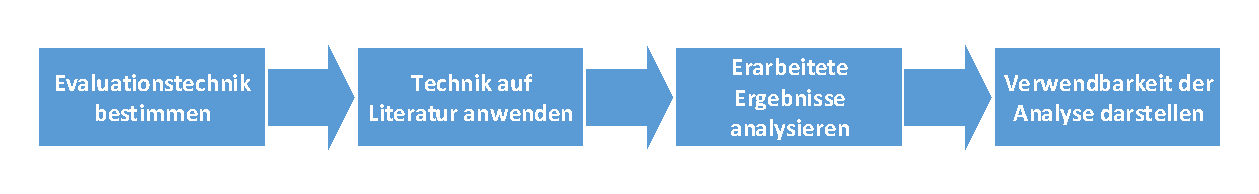
\includegraphics[width=\textwidth]{img/Aufbau_grob.pdf}
  \caption{Grober Aufbau der Arbeit}
  \label{fig:aufbaugrob}
\end{figure}


% Kommentar Korf:
% Aus diesem Bild geht hervor, dass Sie Daten evaluieren, ziehen daraus Schlüsse / leiten Anforderungen ab. Und dann ist Schluss. 
% Das bedeutet auch, dass Sie bei der Evaluation eine signifikante Tiefe erreichen müssen. Das beutet eine detaillierte Literaturarbeit, die sich nicht nur auf die Kommunikation 
% im Auto bezieht. Weiterhin müssen Sie die spezifischen Aspekte der Kommunikation im Auto deutlich herausarbeiten. Sie müssen daraus Schlüsse ziehen und diese untermauern.
% Wollen Sie auf realen Daten evaluieren. Dann sorgen Sie jetzt dafür, dass Sie genug Daten haben. Oftmals muss man subjektive Analysen mit konkreten Daten untermauern.

% META ANALYSE? (oder) DATEN AUS SIMULATION?


% Zielsetzung
Diese Arbeit hat zum Ziel Evaluationstechniken in Hinblick auf deren Einsatzfähigkeit im Feld der Visualisierung von Fahrzeugkommunikationsdaten und deren Werkzeuge zu Analysieren. Unter Zuhilfenahme der erarbeiteten Evaluationstechniken wird spezifische Literatur ausgewertet. Damit ist gemeint das hier Literatur speziell aus dem Bereich der Netzwerkvisualisierung ausgewertet wird, mit Hauptaugenmerk auf die Darstellung von Kommunikationsdaten im Fahrzeug. Aus der Analyse der Literatur ergeben sich Anforderungen an Visualisierungen für den Automotive Bereich, welche Aufgearbeitet werden und somit eine Grundlage für die Entwicklung neuer Visualisierungssystemen und Werkzeuge bilden. 
Somit ergeben sich mehrere konkrete Teilziele dieser Arbeit. Es werden geeignete Evaluationstechniken für die Analyse von Werkzeugen und Visualisierungen im Bereich der Visualisierung von Fahrzeugkommunikation erarbeitet. Es werden konkrete Anforderungen für zukünftige und aktuelle Darstellungsformen und die zugehörige Software zusammengestellt.

\iffalse
Es soll eine Evaluation von Informationssystemen und Visualisierungen stattfinden und deren Vergleich mit dem eigenen Prototypen (sowie dessen Erweiterung zu einem Informationssystem(?)). 

\TODO{Auch noch Teile aus Einleitung AW2? Soll RT Ethernet und dass Fahrzeug mit einbezogen werden? Denke Ja.}
\fi

In Kapitel \ref{cha:umfeldanalyse} wird grob das wissenschaftliche und wirtschaftliche Umfeld umrissen. In drei Unterabschnitten werden hier die Grundlagen und angrenzenden Wissensbereiche dieser Arbeit beleuchtet. Es wird dargelegt inwiefern, nach einschlägiger Literatur, die Wahl der richtigen Evaluationsmethode die Qualität der Ergebnisse und der möglichen Schlussfolgerungen beeinflusst. Aktuelle und bewährte Konzepte der eingesetzten Ethernet Netzwerke, sowie deren Methoden zur Visualisierung von Kommunikationsdaten in Bereichen der Flugzeugtechnik, der Automatisierungstechnik sowie der \iffalse\TODO{Schiffstechnik? Bahn? }\fi werden erörtert, als auch die Anforderungen und die Analyse dieser betrachtet. \iffalse \TODO{Das vielleicht mit in Section Evaluation -> Section: Evaluation und Anforderungsanalyse} \TODO{oder: Evaluation und die Bedeutung für Schlussfolgerungen und Anforderungen}\fi
Kapitel \ref{cha:evaluationsbasis} vergleicht verschiedene Evaluationstechniken und erläutert den Aufbau und die Herangehensweise dieser. Im Verlauf des Kapitels wird Aufgrund von verschiedenen Analysen anderer Wissenschaftlicher Ausarbeitungen eine Evaluationsmethode gewählt. Diese wird zur Evaluation für die im Kapitel \nameref{cha:literaturauswertung} vorgestellten akademischen Abhandlungen verwendet. Das oben genannte Kapitel \ref{cha:literaturauswertung} beinhaltet die erwähnte Literaturauswertung, mit Hilfe der erarbeiteten Evaluationstechnik werden diese Arbeiten aufgearbeitet. Das anschließende Kapitel \ref{cha:anforderungsanalyse} greift die in Kapitel \ref{cha:literaturauswertung} gewonnenen Erkenntnisse auf und es werden darauf basierend Anforderungen für die Darstellung von Netzwerkdaten im Fahrzeug-Ethernet erstellt. Aufgeteilt wird dieses Kapitel in drei Schritte. Zunächst werden allgemeingültige Anforderungen vorgestellt, gefolgt von Anforderungen speziell für den Visualisierungsbereich. Im Anschluss werden konkrete Anforderungen an Visualisierungen von Netzwerkdaten im Fahrzeug gestellt. \iffalse Kapitel \ref{cha:auswahlkriterien} \TODO{möglich in Kapitel 5 rein..} \fi
Das Kapitel \ref{cha:anwendungskonzepte_und_bereiche} beschreibt welche Anwendungsmöglichkeiten sich aus der Anforderungsanalyse ergeben und wie, als auch wo, diese Kombiniert und eingesetzt werden können. Kapitel \ref{cha:zusammenfassung_und_fazit} schließt diese Arbeit mit einer Zusammenfassung und einem Fazit ab.
% chapter einleitung (end)

\chapter{Einführung in das Umfeld} % (fold)
\label{cha:umfeldanalyse}
In der \nameref{cha:einleitung} wurde erläutert warum Visualisierungen für die Darstellung der Netzwerkkommunikationsdaten im Fahrzeug wichtig sind. Dieses Kapitel skizziert die Position dieser Arbeit im Bezug auf das wissenschaftliche Umfeld. Der Kernbereich beschäftigt sich mit Visualisierungen aus dem Automotive Bereich. Im speziellen mit Darstellungen für die Kommunikationsdaten und deren Metriken im modernen Automotive Realtime Ethernet. Neben diesem Hauptbereich gibt es mehrere weitere angrenzende Themen, die für die Arbeit von Bedeutung sind. In der folgenden Übersicht \ref{fig:theme_overview} sind diese Bereiche dargestellt. Das Umfeld ist im Wesentlichen in drei Teile gegliedert, Evaluation, Werkzeuge und Visualisierungen sowie Anforderungen und die Analyse dieser. 

\begin{figure}[htbp]
  \centering
  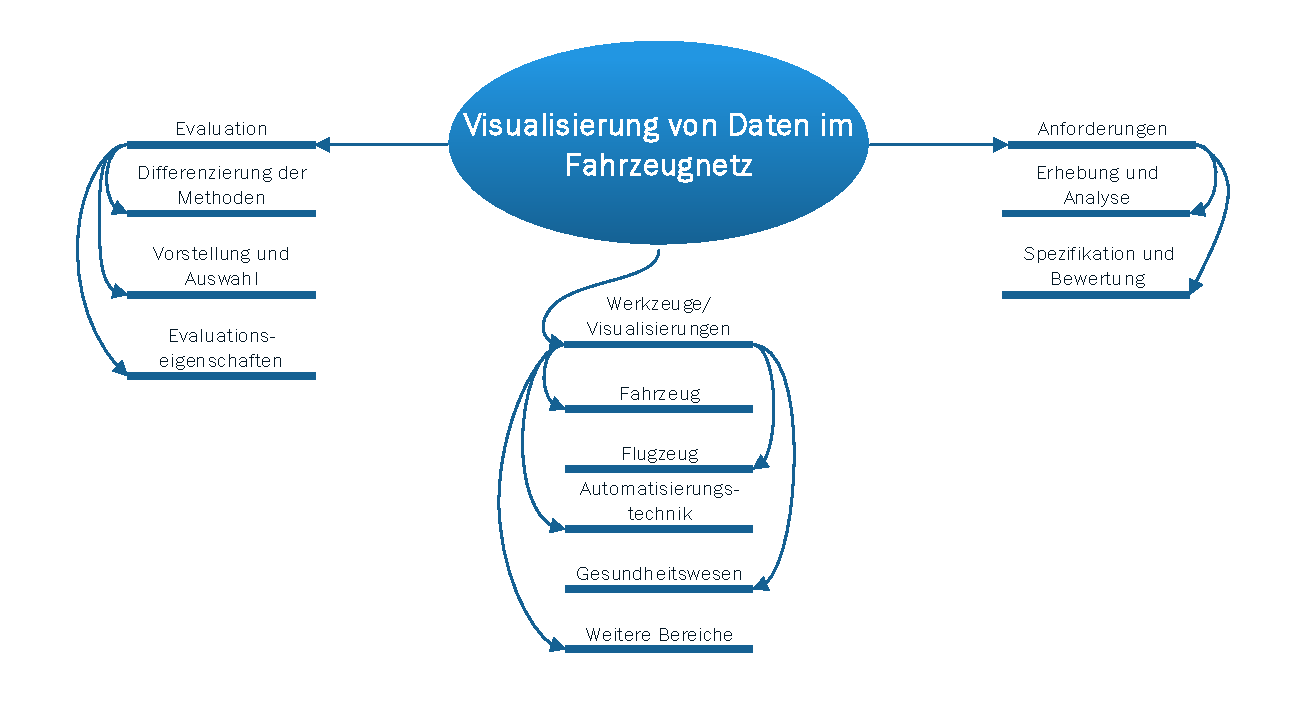
\includegraphics[width=\textwidth]{img/theme_overview.pdf}
  \caption{An diese Arbeit angrenzende wissenschaftliche und wirtschaftliche Bereiche}
  \label{fig:theme_overview}
\end{figure}

Im Abschnitt \ref{sec:grundlagen_der_evaluation} wird benannt welche grundlegenden Evaluationen es gibt und stellt diese vor. Es wird die Vorarbeit für das Kapitel \nameref{cha:evaluationsbasis} geleistet, welches die geeignetste Technik für die Visualisierung von Netzwerkdaten im Fahrzeugnetz herausarbeitet. Abschnitt \ref{sec:visualisierungen_und_werkzeuge} beschreibt die Notwendigkeit der Betrachtung von Visualisierungen und Werkzeugen nicht nur aus dem Automotive Bereich sondern auch aus angrenzenden Bereichen. Der Abschnitt befasst sich weiterhin damit welches diese Bereiche sind und warum diese in Frage kommen. Der abschließende Teil dieses Kapitels, \nameref{sec:anforderungen_und_analyse}, geht auf die Anforderungen an Visualisierungen ein. Es wird \dots 

\section{Grundlagen der Evaluation} % (fold)
\label{sec:grundlagen_der_evaluation}
Im Bereich der Evaluation beschäftigt sich die Arbeit mit der Frage welche Techniken zur Evaluation sinnvoll in diesem Themenkomplex einsetzbar sind. Es wird herausgearbeitet welche Evaluationsmöglichkeiten es gibt und welche, aufgrund Ihrer Ergebnisse und Anwendungsgebiete, am geeignetsten erscheinen. Dieser Abschnitt zeigt grundlegende Evaluationsmethoden und deren Anforderungen sowie nutzen. Im Folgekapitel wird dann eine der vorgestellten Methoden ausgewählt und als Grundlage für die Literaturanalyse verwendet.
Bevor die Techniken zur Evaluation vorgestellt werden, folgt zunächst ein Einblick wie zwischen Evaluationen differenziert wird, weshalb Evaluation verwendet wird und was damit erreicht werden soll.

In der Literatur wird auf verschiedenste Art und Weise zwischen Evaluationen unterschieden. Im folgenden betrachten wir drei verschiedene Klassifikationsarten sowie deren Merkmale, Vorteile und mögliche Nachteile.  
Kitchenham \cite{kitchenham_evaluating_1996-1} hat Mitte der neunziger Jahre bei Evaluierungsmethoden zwischen zwei Messmethodiken differenziert. Zum einen Quantitative Methoden und zum anderen Qualitative Methoden. Eine dritte Variante vereinigt beide Messmethoden, diese werden als Hybride Methoden beschrieben. Die folgende Auflistung beschreibt die genannten Methoden kurz.
\begin{itemize}
  \item Quantitative Methoden, darunter versteht man die Möglichkeit das sich eine messbare Veränderung einer Eigenschaft des zu testenden Softwareprodukts oder Prozesses einstellt. Dabei werden spezifische wissenschaftliche Werkzeuge und Messungen verwendet.
  \item Qualitative Methoden, meinen Feature/Eigenschaften Analysen welche sich auf die Anforderungen an eine bestimmte Aufgabe bzw. Ablauf fokussieren und die Umsetzung dieser Anforderungen innerhalb einer Methode oder eines Tools bewerten.
  \item Hybride Methoden, sind beispielsweise \textit{Qualitative Effect Analysis} oder \textit{Benchmarking}. Die erstgenannte nutzt Quantitative Methoden sowie ein oder mehrere Expertenmeinungen. Beim Benchmarking werden ein oder mehrere Tools einer Reihe von Standardtests unterzogen um die Performance dieser Tools vergleichbar zu machen.
\end{itemize}
Dieser Ansatz Unterscheidet also nach der Art der Messmethode. Der Vorteil in dieser Unterscheidungsart liegt darin, dass bereits zuvor Identifiziert werden kann ob Messbare Effekte bei der Evaluation entstehen oder es sich um eine Eignungsanalyse von Methoden oder Werkzeugen zur Bestimmung der Nutzbarkeit handelt. Dabei können jedoch wichtige Aspekte außer Acht gelassen werden, wie zum Beispiel der nötige Zeitaufwand oder zu welchem Zeitpunkt der Entwicklung eines Programms oder eines Designs die Evaluation am sinnvollsten eingesetzt werden kann. 
In der Psychologie wird bei Evaluationen häufig zwischen formativer und summativer Evaluation unterschieden \TODO{cite}. Es gibt für diese Möglichkeit zur Differenzierung jedoch auch Beispiele aus der Informationsvisualisierung \cite{andrews_evaluating_2006}. 
\begin{itemize}
  \item Formative Evaluation, die formative Evaluation wir meist begleitend zur Implementierung oder zum Projekt durchgeführt. Es wird dabei in Intervallen Untersucht und Zwischenergebnisse festgehalten. So können laufende Prozesse angepasst werden und wiederum erneut evaluiert werden.
  \item Summative Evaluation, als summative Evaluation wird eine das Resultat analysierende Evaluation bezeichnet. Daraus folgt, diese Evaluationen werden nach Abschluss eines Projektes durchgeführt. So ist es möglich das Projekt, Design oder ähnliches zusammenfassend zu bewerten.
\end{itemize}
Eine Unterscheidung zwischen Methoden welche während oder nach einem Projekt durchgeführt werden, erscheint besonders dann sinnvoll wenn vor einem Projekt festgelegt wird mit welchen Methoden während und abschließend gearbeitet werden soll. Da in dieser Arbeit bestehende Visualisierungen auf ihre Eignung für den Einsatz in einer möglichen Automotive Ethernet Netzwerkvisualisierung hin Evaluiert werden, fallen formative Methoden bereit von vornherein aus. So kann also gesagt werden das diese Art der Unterscheidung sich nicht für die Ziele dieser Arbeit eignet. 

Die letzte Differenzierung die hier betrachtet werden soll, unterscheidet
grundsätzlich zwischen zwei Herangehensweisen für Evaluationen. Zum Einen aus der Sicht des Experten in Hinblick auf Softwaredesigns oder der Usability, ohne Einwirkung von Nutzern. Das sind sogenannte Prüfmethoden. Zum anderen Evaluationen die die tatsächliche Nutzung eines Systems untersucht, namentlich Testmethoden, in welchen repräsentative Endnutzer ein oder mehrere Interfaces nutzen und Beobachtungen oder Messungen aufgezeichnet werden.
\begin{itemize}
  \item Evaluation durch Expertenanalyse, dies basiert auf anerkannten Expertenmeinungen mit Hilfe welcher das Design bewertet wird und die Auswirkungen auf Nutzer analysiert werden.
  \item Evaluation durch Nutzermitwirkung, lässt den Endanwender das System auf verschiedene Art und Weisen testen. Die Usability steht im Vordergrund.
\end{itemize}
Ersteres eignet sich insbesondere zur Bewertung von Design, Darstellung und Prototypen, letzteres benötigt normalerweise einen funktionierenden Prototypen oder eine bereits bestehende Implementierung. Natürlich ist das eine sehr grobe Unterscheidung und es kann dabei zu Überschneidungen kommen. Beispielsweise können Nutzer bereits im frühen Entwicklungsprozess mit eingebunden werden oder Experten basierende Analysen werden an bestehenden Implementierungen durchgeführt um günstig und vor allem schnellere Usability Bewertungen vornehmen zu können. Der grobe Unterscheidungsgrad dieser Aufteilung eignet sich gut um ein weites Spektrum an Evaluationen zu betrachten. Diese Differenzierung erscheint, auf Grund der genannten Vorteile beider Evaluationsarten, am geeignetsten für die Arbeit. Bevor die wesentlichen, in diese Aufteilung passenden, Evaluationen vorgestellt werden, werden zunächst noch die allgemeinen Ziele von Evaluationen betrachtet.
% Diese Ausarbeitung nähert sich einer Evaluation aus der Sicht der Usability.

\subsection{Evaluationsziele} % (fold)
\label{sub:evaluationsziele}

% subsection evaluationsziele (end)
Für Evaluationen können, laut Dix \cite{alan_dix_human-computer_2004}, drei Hauptziele genannt werden. Zu nächst den Umfang und die Erreichbarkeit der Funktionalitäten des Systems zu bewerten, die Bewertung der Benutzererlebnisses und spezifische Probleme des Systems zu identifizieren. Die Funktionalität ist wichtig, weil sie den Erwartungen und den Anforderungen des Nutzers entsprechen muss und ihn bei seiner beabsichtigten Aufgabe zu unterstützen. Anders ausgedrückt, sollte das Design den Benutzer dazu bemächtigen seine Aufgabe leichter zu erledigen. Das bedeutet nicht nur, dass die passende Funktionalität vom System her gegeben ist, sondern auch das diese leicht erreichbar ist. Dies ist gemeint, im Sinne von Aktionen die ein Nutzer ausführen muss um die gewünschte Aufgabe erledigen zu können.
Zusätzlich zur Analyse der Funktionalität gibt es die Analyse der  Nutzererfahrung bei der Interaktion mit dem System. Das beinhaltet Aspekte wie die Zufriedenheit des Nutzers mit dem System, wie einfach es zu erlernen ist oder eben die Usability. Weiterführende Punkte können auch den Spaßfaktor und emotionale Reaktionen umfassen, speziell bei Systemen welche zur Unterhaltung oder Entspannung gedacht sind. 
Das dritte Ziel von Evaluationen, ist Probleme mit dem Design zu identifizieren. Das können Ausprägungen sein wie, unvorhergesehenes Verhalten von bestimmten Funktionen des Designs oder Funktionen welche den Nutzer verwirren. Die beiden erstgenannten Ziele, Funktionalität und Usability des Designs, haben natürlich Einfluss auf dieses Ziel. Trotzdem ist dies ein eigenständiges Ziel, da es sich spezifisch auf die Identifikation von Fehlerquellen und Konflikten bezieht, welche dann korrigiert werden können.

\subsection{Evaluationstechniken basierend auf Expertenanalyse} % (fold)
\label{sub:evaluationstechniken_basierend_auf_expertenanalyse}

Idealerweise beginn die Evaluation bei Software, Design oder Projekten bereits bevor jegliche Implementation stattfindet, also in der Design- und Entwicklungsphase. Wenn bereits das Design selbst evaluiert wird, können schwerwiegende und möglicherweise kostenintensive Fehler vermeidet werden. Denn so kann das Design noch angepasst werden bevor zu viele Ressourcen darauf verwendet werden. Typischerweise sind Designfehler umso teurer je später im Entwicklungsprozesses sie entdeckt werden und damit die Wahrscheinlichkeit geringer das diese korrigiert werden können. Allerdings sind regelmäßige Usertests während der Entwicklungsphase teuer und es ist kann sich als schwierig erweisen eine akkurate Bewertung der Interaktionserfahrung der User über ein nicht vollständiges System zu bekommen. Die Konsequenz daraus ist, dass einige Methoden entwickelt wurden um Systeme von Experten evaluieren zu lassen. Diese wiederum können nicht nur verwendet werden um während der Entwicklung bewertend einzugreifen, sondern auch nach der Veröffentlichung um eine Qualitäts- oder Eignungsbewertung vorzunehmen. Im Grunde können diese Methoden zu jedem möglichem Zeitpunkt im Entwicklungsprozess eingesetzt werden, von der Spezifikation des Designs über Prototypen sowie eben auch vollständigen Implementationen, was sie zu einem sehr flexiblem Ansatz zur Evaluation macht. Der Aspekt, der Flexibilität und der Möglichkeit vollwertige Implementationen zu untersuchen, ist besonders relevant für diese Arbeit. Es unterstützt den Ansatz der Arbeit bestehende Visualisierungen auf ihre Eignung zur Darstellung von Netzwerkkommunikationsdaten im Automotive Ethernet Netzwerk zu präsentieren. Die Möglichkeit der Evaluation während der Entwicklung hingegen nicht weiter betrachtet, da diese nicht relevant ist. Expertenanalysen hängen davon ab, dass Designer, Analysten oder Domänenexperten, Design und Darstellungen betrachten und bewerten wie sich dieses auf den typischen User auswirkt. Die grundlegende Intension ist Teile der Software oder des Designs beziehungsweise der Visualisierungen zu identifizieren welche sich nicht an Kognitive Prinzipien halten oder bestätigte empirische Untersuchungen ignorieren. Was diese Methoden nicht betrachten ist die tatsächliche Nutzung des Systems, es kann nur analysiert werden ob Usability Standards eingehalten werden.
Nachfolgend werden aus dem Bereich der Expertenanalyse folgende Ansätze vorgestellt: 

\begin{itemize}
  \item \nameref{ssub:cognitive_walkthrough}
  \item \nameref{ssub:heuristische_evaluation}
  \item \nameref{ssub:modellbasierte_evaluation}
  \item \nameref{ssub:verwendung_von_vorangegangenen_studien}
\end{itemize}

\subsubsection{Cognitive walkthrough} % (fold)
\label{ssub:cognitive_walkthrough}

% subsubsection cognitive_walkthrough (end)

\subsubsection{Heuristische Evaluation} % (fold)
\label{ssub:heuristische_evaluation}
Vorgestellt wurde die heuristische Evaluation von Nielsen und Molich \cite{nielsen_heuristic_1990} 1990. Es handelt sich dabei um eine Usability Untersuchung in welcher jedes Element eines User Interfaces auf bestimmte Usability-Prinzipien hin untersucht wird. Bevor diese Prinzipien entwickelt wurden, wurde die Heuristische Evaluation, im Allgemeinen, basierend auf Intuition und allgemein anerkannten Methoden aufgebaut. Da Heuristische Evaluation bereits auf Design Spezifikationen angewendet werden kann eignet es sich bereits zur Auswertung von frühen Designphasen. Allerdings kann diese Art der Evaluation auch auf Prototypen, Konzepte und bereits voll funktionsfähige Systeme angewendet werden. Daher ist Heuristische Evaluation ein flexibler und günstiger Ansatz. Aufgrund dieser Attribute wird es auch häufig als Discount Usability Methode bezeichnet \cite{kane_finding_2003}\cite{nielsen_usability_1994}.
Generell gibt es bei Heuristischer Evaluation die Vorgabe dass mehrere Auswerter  ein System, unabhängig von einander, beurteilen und mögliche Usabilityprobleme aufzeigen. Es ist entscheidend das es mehrere Auswerter gibt und auch das diese unabhängig von einander dass System evaluieren. Nielsen fand in seiner Abhandlung heraus das drei bis fünf Auswerter ausreichend sind. Bei einer Anzahl von fünf Auswertern, werden im Schnitt 75\% aller Usabilityprobleme gefunden. Wohingegen einzelne Auswerter nur zwischen 20 und 51\% finden konnten, bei mehr als zehn Auswertern ist keine Steigerung der gefundenen Usabilityprobleme mehr zu erkennen.
Um die Auswerter bei der Evaluation zu unterstützen gibt es zehn vorgegebene Heuristiken \cite{nielsen_usability_1994}. Diese können, wenn nötig, um Domänenspezifische Heuristiken ergänzt werden. Für die Darstellung von Netzwerkdaten im Automotive Ethernet Bereich, wären beispielsweise \textit{Erkennbarkeit einschlägiger Metriken} eine mögliche Ergänzung. 
Jeder Auswerter bewertet das System und notiert jeden Verstoß gegen eine der vorgegebenen Heuristiken, welcher ein potentielles Usabilityproblem aufzeigt. Zu jedem Fund wird die schwere des Problems oder des Verstoßes festgehalten. Diese Einschätzung basiert auf vier Faktoren.

\begin{enumerate}
  \item Wie häufig tritt das Problem auf
  \item Wie einfach ist es für den User dieses zu überwinden
  \item Tritt es einmalig auf oder ist es reproduzierbar
  \item Als wie schwer wird das Problem wahrgenommen
\end{enumerate}

Diese werden auf einer Skala von 0 - 4 bewertet. 

\begin{itemize}
  \item[] 0 = Es ist kein Usabilityproblem
  \item[] 1 = Kosmetisches Problem, nicht zwingend zu bearbeiten
  \item[] 2 = kleines Usabilityproblem, niedrige Priorität
  \item[] 3 = großes Usabilityproblem, hohe Priorität
  \item[] 4 = kritisches Usabilityproblem, muss vor Veröffentlichung gelöst werden 
\end{itemize}

Die zehn oben angesprochenen Heuristiken sind:

\begin{enumerate}
  \item 
\end{enumerate}

Zusammenfassend...
Heuristic evaluation involves having a small set of evaluators examine the interface and judge its compliance with recognized usability principles (the "heuristics").

% subsubsection heuristische_evaluation (end)

\subsubsection{Modellbasierte Evaluation} % (fold)
\label{ssub:modellbasierte_evaluation}

% subsubsection modellbasierte_evaluation (end)

\subsubsection{Verwendung von vorangegangenen Studien} % (fold)
\label{ssub:verwendung_von_vorangegangenen_studien}

% subsubsection verwendung_von_vorangegangenen_studien (end)
% subsubsection evaluationstechniken_basierend_auf_expertenanalyse (end)

\iffalse
Neben der Unterteilung in diese drei Bereiche, gibt es eine weitere Dimension bei einer Evaluierung, die Art wie eine Evaluierung aufgebaut ist. Auch hier wird zwischen drei möglichen Typen unterschieden:

\begin{itemize}
  \item Formales Experiment, als formales Experiment bezeichnet man den Vorgang in dem von den Nutzern verlangt wird eine bestimmte Aufgabe, oder auch verschiedene, auszuführen unter Zuhilfenahme der zu untersuchenden Werkzeuge oder Methoden. 
  \item Fallstudie, hier wird jede Methode oder jedes Werkzeug in einem Projekt aus der Praxis getestet. Dabei werden die Standardentwicklungsprozeduren der evaluierenden Organisation verwendet.
  \item Umfrage, Nutzer welche zuvor bestimmte Methoden oder Werkzeuge verwendet haben werden nach Ihren Erfahrungen mit diesen befragt. Die Informationen der Benutzer können dann mit statistischen Techniken analysiert werden.

  \TODO{Add expert eval approaches from eval techniques in HCI Book, nochmal schauen in kitchenham wegen weiteren sachen}
\end{itemize}

\TODO{Korf: Anforderungen an diese Methoden und was kann man daraus gewinnen}

Die genannten Bereiche können mit verschiedensten Typen der Evaluation kombiniert werden.

4. Qualitative screening: A feature-based evaluation done by a  single individual who not only determines the features to be assessed and their rating scale but also does the assessment. For  initial screening, the evalua- tions are usually based  on literature describing the soft- ware method/tools rather than actual use of the meth- ods/too KITCHENHAM1

\begin{itemize}
  \item scope of eval: prototype , e.g., to see if a visualization has achieved
its design goals, to see how a prototype compares with
the current state-of-the-art systems or techniques.
\end{itemize}
\TODO{...}
\TODO{Beispiele}
\fi

\subsection{Evaluationstechniken mit Nutzerbeteiligung} % (fold)
\label{sub:evaluationstechniken_mit_nutzerbeteiligung}

% subsection evaluationstechniken_mit_nutzerbeteiligung (end)
% section grundlagen_der_evaluation (end)

\section{Einführung in grundlegende Visualisierungen und Werkzeuge} % (fold)
\label{sec:visualisierungen_und_werkzeuge}

Visualisierungen und Werkzeuge wie zum Beispiel Informationssysteme werden in vielen Bereichen der Wissenschaft und Wirtschaft eingesetzt. Dieser Abschnitt möchte einen Überblick über Methoden und Werkzeuge geben und dabei auch in angrenzende Wissensbereiche vorstoßen. 

Um numerische Daten in konkreten Visualisierungen festzuhalten eignen sich räumliche Positionsangaben, laut graphischen Wahrnemungsexperiementen, am besten \cite{heer_tour_2010}. Bereits 1786 entwickelte William Playfair die noch heute weit verbreiteten, positionskodierten, Balken- und Liniendiagramme \cite{playfair_playfairs_1768}. Zur Visualisierung von, beispielsweise verfügbarer und/oder genutzter Bandbreite bieten diese Darstellungen noch immer einen angemessenen Informationsgehalt. Diese gehören weiterhin zu den Standarddarstellungsformen, nicht nur für Netzwerkdaten. Ebenso weit verbreitet ist das, ebenfalls von Playfair entwickelte, Kreisdiagramm (auch als Torten- oder Kuchendiagramm bekannt) zur Darstellung von Teilwerten eines Ganzem \cite{playfair_statistical_1801}. Ein Kreisdiagramm kann beispielsweise Verwendung finden um die genutzte Bandbreite verschiedener Links darzustellen. 

Weitere naheliegende Darstellungsarten sind die der Netzwerkvisualisierungen. In diesen werden Beziehungen zwischen Daten aufgezeigt. Das kann sowohl in sozialen als auch in physischen Netzwerken sinnvoll sein, aber auch für Datenbanken oder auch Unternehmensstrukturen. Im mathematischen Sinne sind Netzwerke Graphen und bestehen im Grunde aus zwei primitiven Elementen, Knoten und Kanten, wobei die Kanten die Knoten verbinden. Ein zentraler Punkt bei der Visualisierung mit Graphen stellt die Auswahl eines effektiven Layouts sowie der gewünschte Detailgrad der Analyse dar. Typischerweise werden stark verbundene Knoten auch im Bild nah aneinander positioniert, ebenso werden nicht verwandte Knoten weiter voneinander entfernt platziert, um die Beziehungen differenzieren zu können. Im folgenden werden einige mögliche Netzwerkvisualisierungen besprochen.

\TODO{Zwei gängigere Methoden noch.}

\textbf{Force-directed Layout.}  Bei diesem Layout wird der Graph als physisches System modelliert. Knoten sind geladene Partikel welche sich gegenseitig abstoßen, die Verbindungen zwischen diesen fungieren als Federn und halten die Knoten zusammen. Mit Hilfe einer physischen Simulation dieser Kräfte (forces), werden die Positionen der Knoten festgestellt. Hinzu kommt das der Nutzer mittels Interaktivität das Layout ordnen kann wobei die physikalischen Eigenschaften beibehalten werden. Entwickelt wurde dieses Modell von Fruchtermann und Reingold \cite{Fruchterman91graphdrawing}. 

\textbf{Matrix View.} Ungerichtete Graphen können mathematisch als Adjazenzmatrix beschrieben werden. Für ein Netzwerk, im Grunde ein ungerichteter Graph, bietet es also an eine solche Darstellung zu verwenden. Jeder Wert in Zeile \textit{i} und Spalte \textit{j} in der Matrix korrespondiert zu der Anzahl der Links von Knoten \textit{i} zu Knoten \textit{j}. Ghoniem und Fekete beschreiben beispielsweise in Ihrer Abhandlung die Implementation dieser Technik \cite{Ghoniem:2003:MVG:1063669.1063698}.

Eine noch detaillierte Einführung in die Netzwerk-Analyse mit Hilfe von Graphen bietet die Arbeit von Brandes et. al \cite{brandes2005network}. \TODO{Details hier her?}
\ldots

Mengen mit Werten die sich über die Zeit verändern, sind eine der häufigsten Formen von aufgezeichneten Daten. Auch im Netzwerk häufen sich Daten welche über die Zeit veränderlich sind, wie die genutzte Bandbreite, die Veränderung der Latenz oder des Jitters. Es gibt einige Visualisierungen die diese Art der Darstellung von sogenannten Time-Series Data/Zeitreihendaten unterstützen. 

\textbf{Small Multiples.} Mehrere Zeitreihen können innerhalb von nur einem Diagramm dargestellt werden. Dadurch können allerdings Überschneidungen entstehen wodurch sich die Lesbarkeit verringern kann. Eine Alternative ist die Darstellung in Small Multiples, hier wird jede Zeitreihe Achsen-gleich in einem eigenen Diagramm dargestellt. Durch diese Darstellung können allgemeine Trends sowie individuelle Muster erkannt werden. In Projekt 1 wurde diese Darstellungsform bereits in kleinem Rahmen gewährleistet. \iffalse Wie in Abbildung \ref{fig:synch_splines} zu sehen, können über einen Synchronisationsbutton die verschiedenen Zeitreihen auf eine einheitliche Skala des höchsten Maximums und des kleinsten Minimums der ausgewählten Diagramme angepasst werden.
\begin{figure*}[htbp]
  \centering
  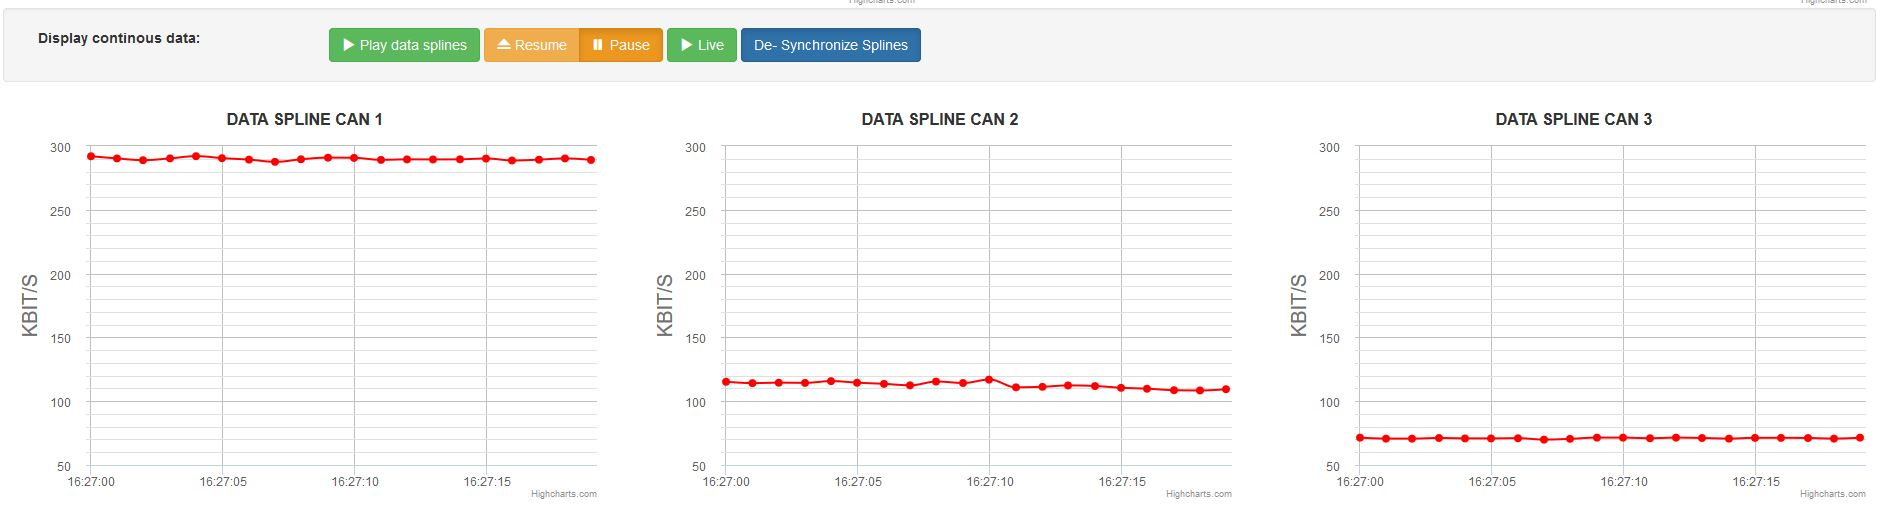
\includegraphics[width=\textwidth]{img/synch_splines}
  \caption{Small Multiples der genutzten Bandbreite von drei verschiedenen CAN-Bussen}
  \label{fig:synch_splines}
\end{figure*}
\fi

In Burch und Weiskopfs Abhandlung \cite{Burch:2014:FES:2636240.2636839} wird diese Darstellungsform zur Verdeutlichung der Dynamik von Graphen genutzt. Im Small Multiple Aufbau werden Node-Link Diagramme verwendet, welche die Veränderung des Graphen Sequentiell vermitteln soll. Die Vorteile eines Small Multiple Aufbaus gegenüber, von den Autoren als sogenannte Large Singles bezeichnete, einfachen Darstellungen wird in van den Elzen und van Wijks Artikel erläutert \cite{elzen_small_multiple_2013}. Die Kernaussage besagt, dass mit Small Multiples ein breiterer Umfang an Daten aufgenommen werden kann als mit Lage Singles.

\textbf{Index Charts.} Für einige Zeitreihen ist die relative Veränderung ausschlaggebender als die tatsächliche Veränderung der Daten. Für diese Daten kommt ein Index Chart in Frage. Dieser Diagrammtyp zeigt die prozentuale Veränderung für eine Sammlung von Zeitreihen basierend auf einem fixen indexiertem Punkt \cite{heer_tour_2010}. Diese Diagrammart kann beispielsweise bei der Visualisierung von Netzwerkdaten eingesetzt werden um bei einer Verbindungen festzustellen wie sich die Last ab einem bestimmten Zeitpunkt prozentual erhöht. Als Zeitpunkt in einem Fahrzeug beispielsweise das Anlassen des Motors. So lässt sich analysieren welche Verbindungen den größten prozentualen Lastzuwachs, ab diesem Zeitpunkt, erfahren.

\ldots
Naheliegender angrenzende Bereiche sind jene aus dem Verkehrswesen. In der Flugzeugtechnik wird bereits mit Ethernet im Flugzeugnetz experimentiert und es ist auch schon im Einsatz, beispielsweise im A380 oder der Boeing 787. Auch hier wurde der erhöhte Kommunikationsbedarf erkannt und mit einem auf die Luftfahrt spezialisiertem und von Airbus entwickelten Datennetz reagiert. Das sogenannte Avionics Full-Duplex Switched Ethernet (AFDX) wird hauptsächlich für sicherheitskritische Anwendungen verwendet \cite{steiner_recent_2014}. 


% section visualisierungen_und_werkzeuge (end)

\section{Grundlagen für Anforderungen und Analyse} % (fold)
\label{sec:anforderungen_und_analyse}
Dieser Abschnitt beschreibt grundlegende Aspekte ... 

Damit visuelle Analyse Tools effektiv genutzt werden können, müssen diese eine fließende und flexible Nutzung von Visualisierungen ermöglichen. Um das zu ermöglichen wird in \cite{heer_interactive_2012} eine \textit{Taxonomy of interactive dynamics for visual analysis} eingeführt. Diese ist in drei Kategorien eingeteilt welche die kritischen Aufgaben der visuellen Analyse beschreiben. Die Kategorien sind \textit{Data and View Specification}, \textit{View Manipulation} sowie \textit{Process and Provenance}. Die erste Kategorie beschäftigt sich mit den spezifischen Daten und Views welche für die jeweiligen Bedürfnisse der Analysten von Interesse sind. Es muss eine Steuerung der Applikation ermöglicht werden, so dass die Daten selektiv visualisiert werden können, irrelevante Daten herausgefiltert werden und ebenso müssen die Informationen sortiert werden können um mögliche Muster erkennbar zu machen. Nach der Erstellung einer Visualisierung muss es den Analysten ermöglicht werden die gestellten Views nach Bedürfnis zu manipulieren, dies beschreibt die zweite Kategorie der Taxonomy. Die Manipulation der Visualisierung ist nötig um Muster aufzeigen zu können, Hypothesen zu untersuchen und zur Navigation in den Daten bspw. via Drilldown. Analyse Tools muss es möglich sein multiple verbundene Visualisierungen zu organisieren und zu koordinieren um mehr Einsicht in Multidimensionale Daten zu bieten als es isolierte Views vermögen. Dies wird schon im häufig zitierten Mantra von Ben Shneiderman vorgegeben: "\textit{Overview first, zoom and filter, then details-on-demand}" \cite{shneiderman_the_eyes_1996}. Die abschließende Kategorie \textit{Process and Provenance} beschreibt den iterativen Prozess der Datenexploration sowie den der Dateninterpretation. Wenn Analysten Ihre bisher getätigten Aktionen innerhalb eines Programms nachverfolgen können kann die Arbeit überprüft und verbessert werden. Es sollte möglich sein die Ergebnisse zu dokumentieren als auch diese mit anderen zu teilen um eine Diskussion darüber zu ermöglichen. Ferner können Analysewerkzeuge auch Anfänger durch Ihre Funktionen führen um die Benutzung und den Einstieg zu erleichtern.
Die vorgegebene Taxonomie bietet einen guten Einstiegs- und Orientierungspunkt in der Welt der Visualisierung und kann ebenso als Checkliste bei der Entwicklung eines neuen Analysetools verwendet werden. Sie zeigt viele Möglichkeiten auf um den Daten Herr werden zu können. 

% section anforderungen_und_analyse (end)

\chapter{Evaluationsbasis} % (fold)
\label{cha:evaluationsbasis}
In den letzten 20 Jahren beschäftigten sich über 80\% der Evaluationen bezüglich der Visualisierung und ihrer Werkzeuge mit den sich ergebenden Bildern und mit der Performance der verwendeten Algorithmen. Allerdings lassen mehr und mehr Evaluationen Teilnehmer in ihren Studien partizipieren. Von den Teilnehmern wird dann die Leistungen sowie das subjektive Feedback Evaluiert oder es wird ihre (verbesserte) Performance mit der Visualisierung und in der Analyse, als auch bei der Fähigkeit zur Schlussfolgerung berücksichtigt \cite{isenberg_systematic_2013}. 

Die Wahl der Art der Evaluation ist entscheidend, weil diese vorgibt in welcher Art und Weise die Ergebnisse genutzt werden können. Diese Entscheidung wird von mehreren Faktoren beeinträchtigt. Den Zielen welche mit der Methode erreicht werden sollen, die Umstände und Grenzen die der Evaluationsaufgabe auferlegt sind und der Charakteristik der Objekte welche evaluiert werden sollen. Diese unterschiedlichen Faktoren interagieren miteinander was die Wahl der geeignetsten Evaluationsmethode schwierig gestaltet \cite{kitchenham_evaluating_1996-2}.

Lam et al. haben in ihrer Ausarbeitung \cite{lam_empirical_2012} 850 Paper hinsichtlich möglicher Evaluierungsszenarien untersucht. Sie haben sieben verschiedene Szenarien ermittelt, welche sich in zwei grundlegende Kategorien aufteilen. Zum einen gibt es Szenarien, welche mit dem Verständnis der eigentlichen Visualisierungen beschäftigen, zum anderen solche die zum Nachvollziehen der Datenanalyse dienen. Besonders das Szenario aus der Datenanalyse \textbf{evaluating visual data analysis and reasoning (VDAR)} sticht für die angestrebte Arbeit heraus. Evaluationen in diesem Bereich fokussieren sich hauptsächlich darauf ob und wie ein Visualisierungswerkzeug visuelle Analysen und Schlussfolgerungen über Daten zulässt. Mögliche Ergebnisse sind hierbei sowohl Metriken (bspw. Anzahl der Analyseerkenntnisse), als auch subjektives Feedback (bspw. Umfrage über Datenanalysequalität). Meist werden in diesem Bereich Feldstudien genutzt, häufig in der Form von Fallstudien.


\iffalse
Wie Eval andere? -> Kriterien / Nutzen?

Aus verschiedenen Evaluationsmöglichkeiten ergeben sich verschiedene Anforderungen

Evaluierungsszenarien und Evaluierungspraktiken
\fi

\section{Häufig verwendete Evaluationen im Bereich Visualisierung} % (fold)
\label{sec:häufig_verwendete_Evaluationen im Bereich Visualisierung}
Visualisierung/Automotive/Angrenzede
% section häufig_verwendete_Evaluationen im Bereich Visualisierung (end)

\section{Faktoren zur Abgrenzung der Evaluationstechniken} % (fold)
\label{sec:Faktoren zur Abgrenzung der Evaluationstechniken}

% section Faktoren zur Abgrenzung der Evaluationstechniken (end)

\section{Entscheidung für Evaluation} % (fold)
\label{sec:entscheidung_für_Evaluation}
dieser oder die Kombi aus diesen ist für Automotive am besten weil! Und dieser wird für die Literaturanalyse bzw. Analyse von bestehenden Visualisierungen und Werkzeugen verwendet.
% section entscheidung_für_Evaluation (end)
% chapter evaluationsbasis (end)

\chapter{Literaturauswertung} % (fold)
\label{cha:literaturauswertung}

Dieses Kapitel beleuchtet die für diese Arbeit relevante Literatur. Das Kapitel ist in zwei Bereiche gegliedert, zum einem werden theoretische Abhandlungen betrachtet welche sich mit Anforderungen an vornehmlich Netzwerk bezogenen Visualisierungen beschäftigen. Zum Anderen...

\section{Verwandte Arbeiten} % (fold)
\label{sec:verwandte_arbeiten}
\iffalse
In einer Studie von Sedlmair et al. \cite{sedlmair2009} wurden ausgewählte Darstellungsarten auf ihren Zuspruch für ein Expertenpublikum getestet. Besonders hervorzuheben ist hier der neu kreierte Autobahnview. Der Autobahn View zeigt den Datenstrom der Bussysteme (die Autobahn). Jeder Bus transportiert Nachrichten verschiedener ECUs, dargestellt als horizontale Linie (eine Fahrbahn der Autobahn). Wobei die Daten als Nachrichten, in Form von kleinen Rechtecken (die Fahrzeuge), dargestellt werden. Adaptiert auf ein Ethernet-Backbone Netz, wären die Virtuellen Links die Autobahn, ein einzelner Link eine Fahrbahn und genauso wie ursprünglich wäre eine Nachricht ein Fahrzeug. Damit lassen sich beispielsweise der zyklische Datenverkehr beobachten, das Verständnis für Fahrzeugnetze erweitern, Ursache-Wirkung Relationen untersuchen sowie die gesamte Fahrzeugkommunikation beobachten. Aufgrund der starken Nachfrage und der großen Breite an möglichen Anwendungsgebieten für die Autobahn Darstellungsform, ist es ein Ziel diese in der nächsten Version des Prototypen, möglicherweise in der  anschließenden Masterarbeit, zu verwirklichen. \TODO{Rewrite, has to be included}
% section verwandte_arbeiten (end)
\fi
\section{Visualisierungen und Werkzeuge} % (fold)
\label{sec:anwendungen_und_werkzeuge}
Es wurde bereits eine große Zahl an verschiedensten Analyse-Werkzeugen entwickelt. Dieser Abschnitt geht auf die Funktion, die Nutzbarkeit und das Anwendungsgebiet der für diese Arbeit relevanten Programme ein. Die Programme kommen aus den verschiedensten Bereichen, der Automatisierungstechnik, der Flug- und Fahrzeugindustrie so wie weiteren kleineren Bereichen. Es handelt sich dabei sowohl um proprietäre, als auch um wissenschaftlich erarbeitete Anwendungen. 
\iffalse\TODO{RLY? Recap if still true} 

Cardiogram \cite{sedlmair_cardiogram:_2011} ist eine Software, die speziell zur Darstellung von Daten im Automotiven Bereich entwickelt wurde. Es visualisiert Fehler in Prototypen-Tests über Logfiles, welche während reellen Testfahrten entstehen. In dieser Arbeit von Sedlmaier et al. gibt es bereits erste Ansätze zum Umgang mit großen Datenmengen im Gigabyte Bereich, wie automatisierte Datenfilterung und -abstraktion über State Machines sowie automatisierte Fehlererkennung.\TODO{detaillierter}


In der neuesten Arbeit von Lajmi et al. \cite{lajmi_using_2013} wurde Ethernet bereits zur Netzwerkanalyse innerhalb eines Fahrzeugs genutzt. Hier wurde ein Netzwerktool ähnlich zu WireShark, namentlich CableFish, entwickelt. Die Software erkennt bereits neuartige Protokolle der Automobilindustrie, wie z.B. SOME-IP \cite{someip_scalable_2014}, und ist gedacht als Unterstützung für Diagnosetools. Allerdings werden hier zwar mit Hilfe von Ethernet Daten empfangen, es wurden allerdings die Daten der fahrzeugspezifischen Protokolle, wie LIN, CAN und FlexRay in Ethernetpakete verpackt. Des Weiteren wurde dieses Programm bisher nur in einer simulierten Umgebung getestet, hat aber eine verbesserte Echtzeitfähigkeit. Da für wurde ein weiterer Buffer vor der Datenspeicherung eingebaut und so die Anzahl der Systemaufrufe reduziert. \TODO{DETAILS}\fi
% section anwendungen_und_werkzeuge (end)
% chapter literaturauswertung (end)

\chapter{Anforderungsanalyse} % (fold)
\label{cha:anforderungsanalyse}

\iffalse
Wie hilft diese Vis Technik/Werkzeug bei welchem Fehler oder Beobachtung auch immer?

Motivation für diese Anforderung?

80:20! welche 20\% Anf. sind für 80\% der Infos verantwortlich??\newline
->>>> SCALABILITY;STORYTELLING?;EFFECTIV EVAL?

A systematic review -> 2. Absatz in Conclusion \cite{isenberg_systematic_2013} \newline
empirical studies in \cite{lam_empirical_2012}
\fi
\section{Allgemeine Anforderungen} % (fold)
\label{sec:allgemeine_anforderungen}

Dieser Abschnitt soll die unterschiedlichen Anforderungen welche an Visualisierungswerkzeuge, ebenso wie an Visualisierungstechniken gestellt werden, herausarbeiten. Im folgenden werden dann die essentiellen Anforderungen hervorgehoben um in einem letzten Schritt diese auf ihre Anwendbarkeit im Automotivebereich geprüft.


\subsection{Anforderungen an Visualisierungen} % (fold)
\label{sub:anforderungen_an_visualisierungen}

Anforderungen an Visualisierungen:

\begin{itemize}
  \item Verständlichkeit und schneller Zugriff auf Daten
  \item Zeitersparnis bei der Analyse
  \item Kollaboratives Arbeiten
  \item Datenabstraktion, Überblick über Daten
\end{itemize}
% subsection anforderungen_an_visualisierungen (end)

\subsection{Anforderungen an Werkzeuge} % (fold)
\label{sub:anforderungen_an_werkzeuge}

Spez. Anforderungen an Werkzeuge:

\begin{itemize}
  \item Große Datenmengen verarbeiten/Datenexploration 
  \item Neue Erkenntnisse schaffen
  \item Visuelle Analysen mit Schlussfolgerungen über Daten
\end{itemize}
\iffalse
\TODO{ANMERKEN: SEHR SEHR ALLGEMEIN, SINN? }\fi
% subsection anforderungen_an_werkzeuge (end)


% section allgemeine_anforderungen (end)
\section{Automotive spezifische Anforderungen} % (fold)
\label{sec:automotive_spezifische_anforderungen}
Visualisierungen Automotive spezifischer:

\begin{itemize}
  \item Verbesserte temporale Struktur und Orientierung
    \begin{itemize}
    \item schnellere Übersicht
    \item bessere Navigationsmöglichkeiten als in Liste
    \item grobe sowie feine Zeitinformationen nötig
  \end{itemize}
  \item Zugriff auf Rohdaten muss gegeben sein
  \begin{itemize}
    \item Signale, Nachrichten und deren Werte müssen abrufbar sein
    \item Abstraktion kann helfen, aber nicht um Werte aus Rohdaten anzuzeigen
  \end{itemize}
\end{itemize}

Werkzeuge mögliche Evaluierungsrichtungen:

\begin{itemize}
  \item Verständnis der Umgebung und Arbeitspraktiken (In welchem Kontext wird es verwendet? Welche Vis?)
  \item Evaluation der visuellen Datenanalyse und Schlussfolgerungen (Entscheidungsfindung, Hypothesengenerierung, Wie wird das unterstützt?)
  \item 
\end{itemize}
% section automotive_spezifische_anforderungen (end)
% chapter anforderungsanalyse (end)
\iffalse
\chapter{Auswahlkriterien} % (fold)
\label{cha:auswahlkriterien}
\TODO{Das eher als section in Anforderungsanalyse?}
Hier steht das Ergebnis der Anforderungsanalyse. Welche Anforderungen möchte ich anführen für eine Entwicklung von Visualisierungen und Visualisierungswerkzeugen im Fahrzeugnetzbereich.
% chapter auswahlkriterien (end)
\fi
\chapter{Anwendungskonzepte und -bereiche} % (fold)
\label{cha:anwendungskonzepte_und_bereiche}

Würde man es nach dem und dem Ansatz machen wäre das ergebnis so und so

kombiniert man den und diesen Ansatz dann wäre das so

daraus ergibt sich (hoffentlich) ein völlig neuer Ansatz
% chapter anwendungskonzepte_und_bereiche (end)

\chapter{Zusammenfassung und Fazit} % (fold)
\label{cha:zusammenfassung_und_fazit}

% chapter zusammenfassung_und_fazit (end)

\backmatter

\typeout{===== Section: literature}
%% read the documentation for customizing the style
\bibliographystyle{abbrv}
\bibliography{ausarbeitung_haw}

\typeout{===== Section: nomenclature}
%% uncomment if a TOC entry is needed
%%\addcontentsline{toc}{chapter}{Glossar}
\renewcommand{\nomname}{Glossar}
\clearpage
\markboth{\nomname}{\nomname} %% see nomencl doc, page 9, section 4.1
\printnomenclature

%% index
\typeout{===== Section: index}
\printindex

\HAWasurency

\end{document}
